\documentclass{article}
\usepackage{tikz} 
\usepackage[utf8]{inputenc}
\usepackage{amsmath}
\usepackage{listings}
\usepackage{amsfonts}
\usepackage{amssymb}
\usepackage{tabularx}
\usepackage{enumitem}
\usepackage{algorithm}% http://ctan.org/pkg/algorithm
\usepackage[noend]{algpseudocode}% http://ctan.org/pkg/algorithmicx
\usepackage[margin=0.7in]{geometry}
\usepackage{tikz}

\usepackage{graphicx}
\usetikzlibrary{arrows,positioning} 
\usepackage{subcaption}
\thispagestyle{empty}
\usepackage{multicol,caption}
\pgfarrowsdeclarecombine{ring}{ring}{}{}{o}{o}

\DeclareMathOperator{\ringarrow}{\raisebox{0.5ex}{\tikz[baseline]{\draw[ring->](0,0)--(2em,0);}}}

\tikzset{
    %Define standard arrow tip
    >=stealth',
    %Define style for boxes
    observed/.style={
           circle,
           rounded corners,
           draw=black, thick,
           minimum width=2.2em,
           minimum height=2.2em,
           font=\footnotesize,
           text centered,
           },
     latent/.style={
           circle,
           rounded corners,
           draw=black, thick, dashed,
           minimum width=2.2em,
           minimum height=2.2em,
           font=\footnotesize,
           text centered,
           fill=black!10!white
           },
            empty/.style={
           circle,
           rounded corners,
           minimum width=.5em,
           minimum height=.5em,
           font=\footnotesize,
           text centered,
           },
    % Define arrow style
    pil/.style={
           o->,
           thick,
           shorten <=2pt,
           shorten >=2pt,},
    sh/.style={ shade, shading=axis, left color=red, right color=green,
    shading angle=45 }
    
}
   
\begin{document}
\def\ci{\perp\!\!\!\perp} % from Wikipedia

Let $q \in [0,1]^N$ be a fixed vector where $q_i = P(X_i = 1)$. In each time-step $t$ upto a known end point $T$:
 
\begin{enumerate}
\item The learner chooses an $I_t \in \set{1,\ldots, N}$ and $J_t \in \set{0,1}$.
\item Then $X_t \in \set{0,1}^N$ is sampled from a product of Bernoulli distributions, $X_{t,i} \sim \Ber(q_i)$ 
\item The learner observes $\tilde X_t \in \set{0,1}^K$, which is defined by 
\eq{
\tilde X_{t,i} = \begin{cases}
X_{t,i} &\text{if } i \neq I_t \\
J_t & \text{otherwise}\,.
\end{cases}
}
\item The learner receives reward $Y_t \sim \Ber(r(\tilde X))$ where $r:\set{0,1}^K \to [0,1]$ is unknown and arbitrary.
\end{enumerate}


\begin{figure}[h]
\centering
\label{fig:causalStructure}
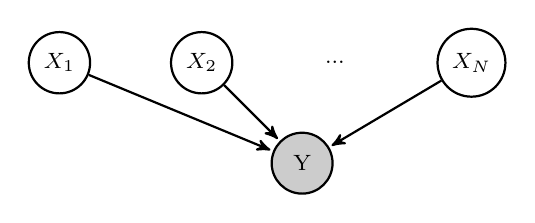
\begin{tikzpicture}[->,>=stealth',shorten >=1pt,auto,node distance=1cm,
  thick,main node/.style={observed}, hidden/.style={empty}]

 %nodes
\node[main node](1){$X_{1}$};
\node[main node, right=of 1](2){$X_{2}$};
\node[hidden, right=of 2](3){$...$};
\node[main node, right=of 3](4){$X_{N}$};
\node[main node,fill=black!20!white, below right=of 2](5){Y};
 \path[every node/.style={font=\sffamily\small}]
    (1) edge (5)
    	(2) edge (5)
    (4) edge (5);
	
\end{tikzpicture}
\end{figure}

\end{document}
